\documentclass[12pt]{article}
\usepackage[rflt]{floatflt}
\usepackage{graphicx}
\pagestyle{empty}
\begin{document}
\openup.5em
\begin{floatingfigure}{2.25in}
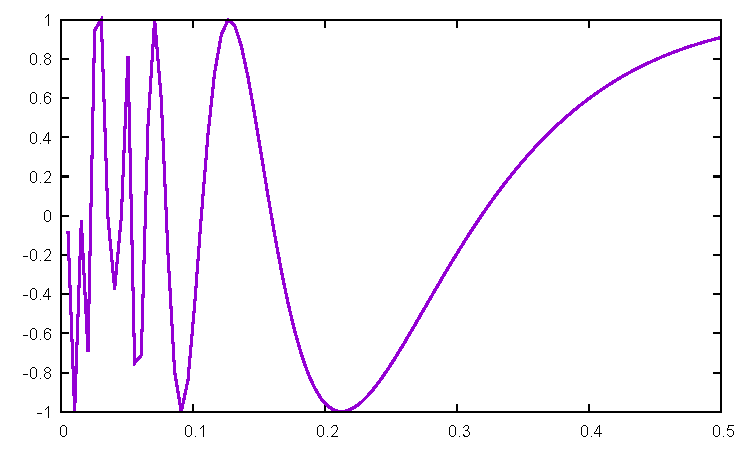
\includegraphics[width=2in]{r2fig}  
\end{floatingfigure}   
It can be difficult to plot functions like $\sin(\frac{1}{x})$ that vary infinitely quickly as $x$ approaches a particular value, in this case $x=0$. 
Unless the function is sampled more frequently than it oscillates, you will produce plotting artifacts, as can be seen in the figure to the right.
In these cases a better result can be obtained by increasing the sample frequency; in gnuplot the command is {\tt set samples 1000}, for example.
\end{document}
